\documentclass{article}

\usepackage{graphicx}
\usepackage{tikz}
\usepackage{tikzsymbols}
\usetikzlibrary{calc,patterns,shapes.geometric}
\pagestyle{empty}
\usepackage[margin=0pt]{geometry}
\geometry{papersize={14in,12in}}

\def\centerarc[#1](#2)(#3:#4:#5){\draw[#1] ($(#2)+({#5*cos(#3)},{#5*sin(#3)})$) arc (#3:#4:#5);}

\begin{document}
	\begin{figure}
		\centering
		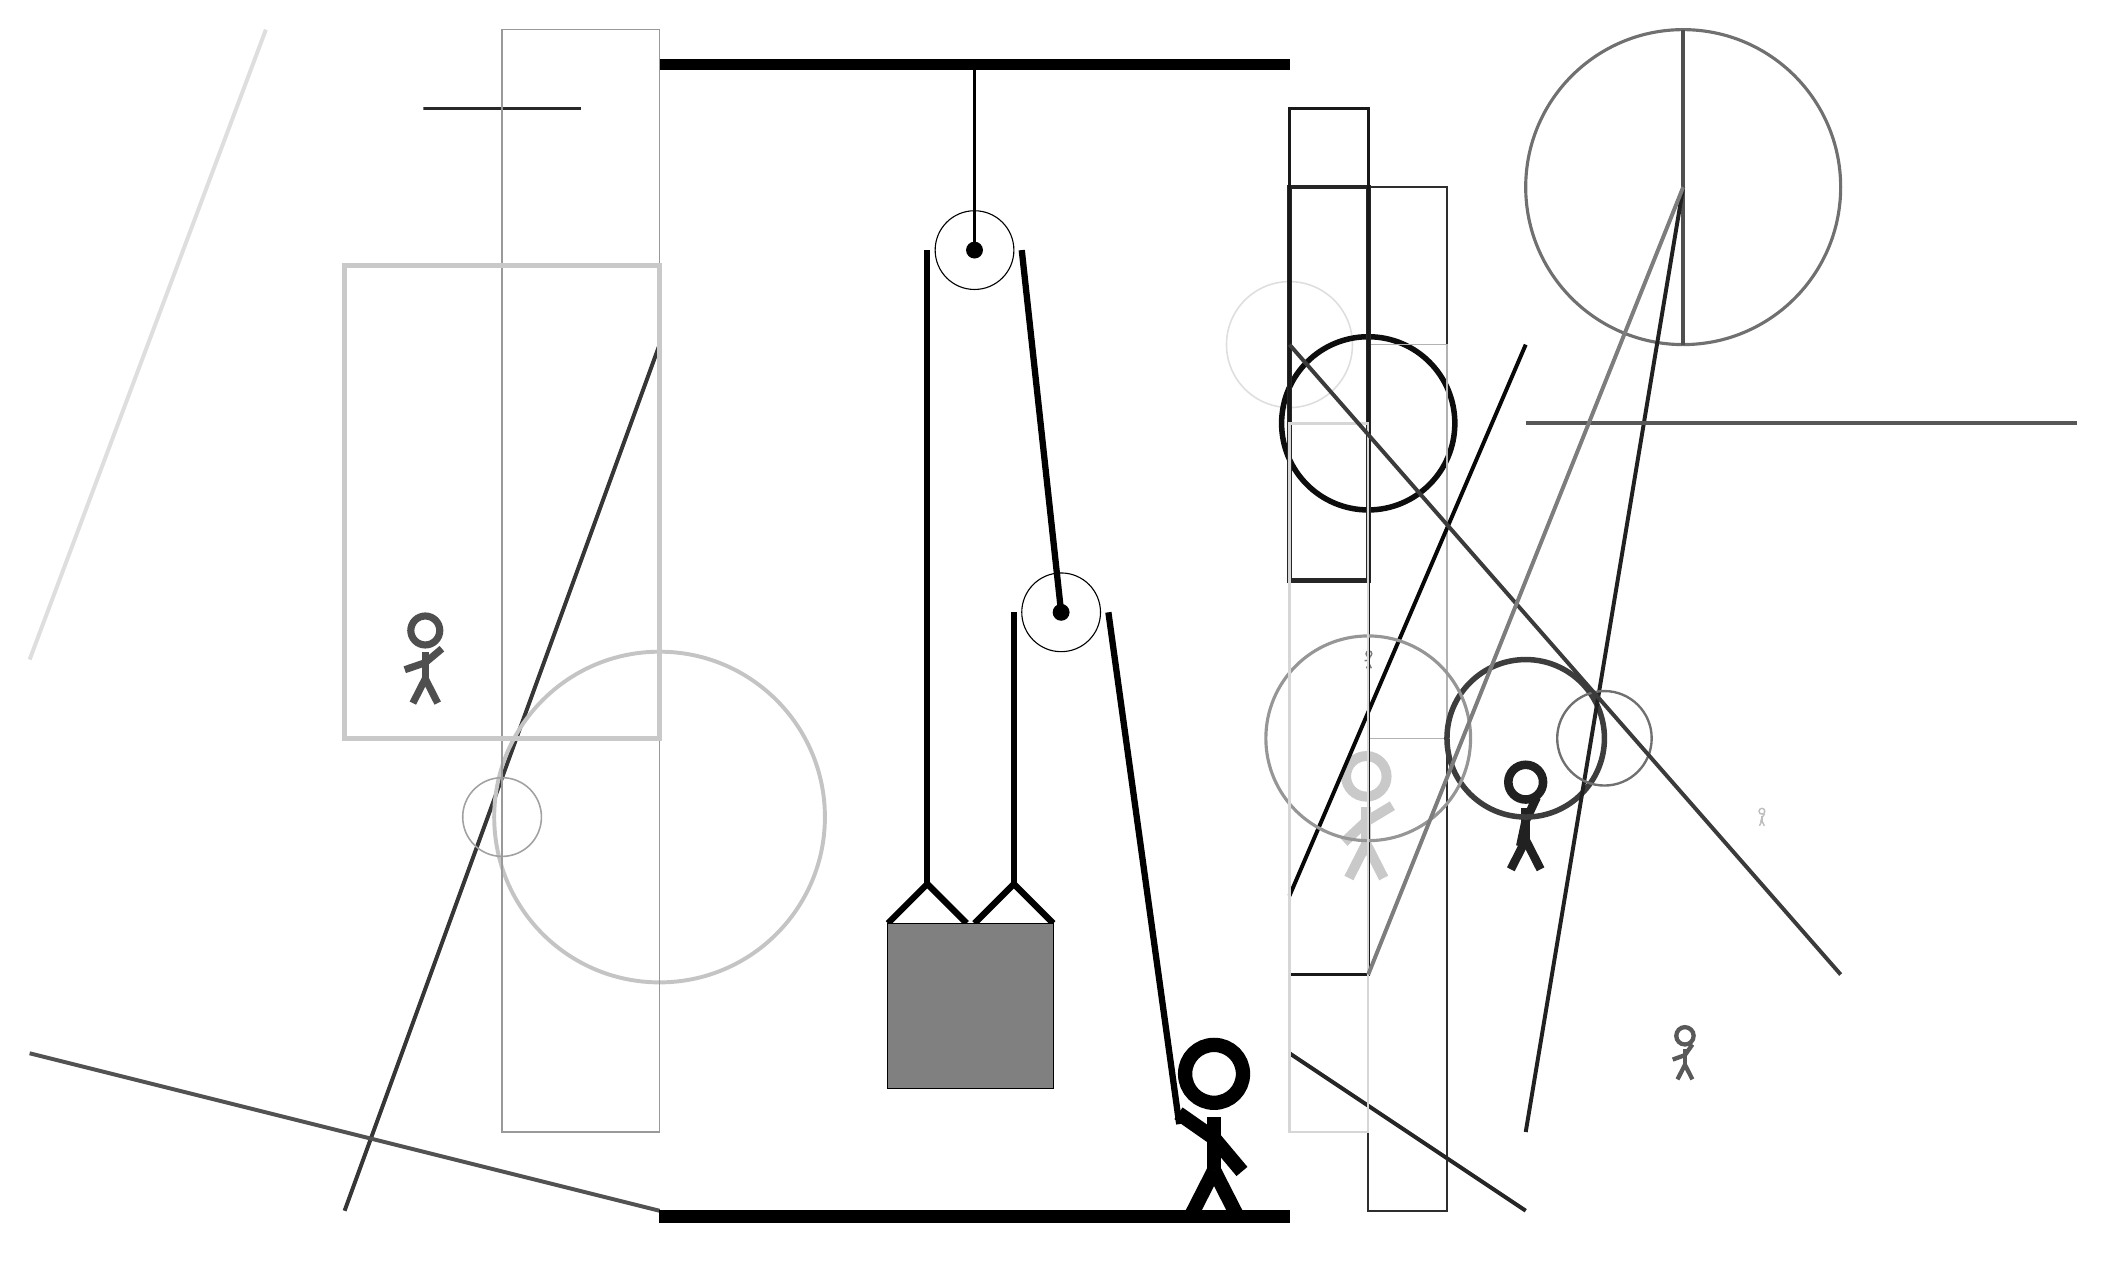
\begin{tikzpicture}
			%%%%% START %%%%%
			
			\draw[fill=black] (-2, 11.5) rectangle (6, 11.625);
			
			\draw[line width=0.5mm, color=black!79](-2, 8) -- (-6, -3);
			
			\node[line width=0.3mm, color=black!21] at (7, 2) {\Strichmaxerl[7][43][31]};
			\draw [line width=0.4mm, color=black!56](11, 10) circle (2.0);
			\draw[line width=0.3mm, color=black!84] (-3, 11) rectangle (-5, 11);
			\node[line width=0.4mm, color=black!69] at (-5, 4) {\Strichmaxerl[5][19][40]};
			
			\draw[line width=0.5mm, color=black!69](11, 12) -- (11, 8);
			\node[line width=0.6mm, color=black!65] at (11, -1) {\Strichmaxerl[3][20][55]};
			\node[line width=0.4mm, color=black!87] at (9, 2) {\Strichmaxerl[6][78][65]};
			\draw [line width=0.2mm, color=black!13](6, 8) circle (0.8);
			\draw [line width=0.7mm, color=black!95](7, 7) circle (1.1);
			
			\node[line width=0.7mm, color=black!26] at (12, 2) {\Strichmaxerl[1][74][54]};
			\node[line width=0.7mm, color=black!52] at (7, 4) {\Strichmaxerl[1][7][72]};
			\draw[line width=0.3mm, color=black!82] (8, 10) rectangle (7, -3);
			
			\draw [line width=0.5mm, color=black!23](-2, 2) circle (2.1);
			\draw [line width=0.2mm, color=black!37](-4, 2) circle (0.5);
			\draw[line width=0.2mm, color=black!30] (7, 3) rectangle (8, 8);
			
			\draw[line width=0.5mm, color=black!97](9, 8) -- (6, 1);
			\draw[line width=0.6mm, color=black!85] (6, 10) rectangle (7, 5);
			\draw [line width=0.7mm, color=black!76](9, 3) circle (1.0);
			\draw[line width=0.5mm, color=black!87](11, 10) -- (9, -2);
			\draw[line width=0.4mm, color=black!90] (6, 11) rectangle (7, 0);
			
			\draw[line width=0.5mm, color=black!85](9, -3) -- (6, -1);
			\draw [line width=0.4mm, color=black!41](7, 3) circle (1.3);
			\draw [line width=0.3mm, color=black!56](10, 3) circle (0.6);
			\draw[line width=0.5mm, color=black!66](9, 7) -- (16, 7);
			\draw[line width=0.2mm, color=black!40] (-4, -2) rectangle (-2, 12);
			\draw[line width=0.3mm, color=black!16] (6, -2) rectangle (7, 7);
			\draw[line width=0.5mm, color=black!77](6, 8) -- (13, 0);
			
			\draw[line width=0.5mm, color=black!68](-2, -3) -- (-10, -1);
			\draw [line width=0.6mm, color=black!30](-8, 4) circle (0.0);
			\draw[line width=0.6mm, color=black!21] (-2, 9) rectangle (-6, 3);
			\draw[line width=0.5mm, color=black!13](-7, 12) -- (-10, 4);
			\draw[line width=0.5mm, color=black!51](11, 10) -- (7, 0);
			
			\draw (2, 9.2) circle (0.5);
			\draw[fill=black] (2, 9.2) circle (0.1);
			\draw[thick] (2, 9.2) -- (2, 11.5);
			
			\draw (3.1, 4.6) circle (0.5);
			\draw[fill=black] (3.1, 4.6) circle (0.1);
			
			\draw[line width = 0.8mm]  (0.9, 0.65) -- (1.4, 1.15) -- (1.9, 0.65);
			\draw[line width = 0.8mm]  (2.0, 0.65) -- (2.5, 1.15) -- (3.0, 0.65);
			\draw[fill=black!50] (0.9, 0.65) rectangle (3.0, -1.45);
			
			\draw[line width = 0.8mm] (1.4, 9.2) -- (1.4, 1.15);
			\centerarc[line width = 0.8mm](2, 9.2)(0:180:0.6);
			\draw[line width = 0.8mm] (2.6, 9.2) -- (3.1, 4.6);
			\draw[line width = 0.8mm] (2.5, 4.6) -- (2.5, 1.15);
			\centerarc[line width = 0.8mm](3.1, 4.6)(0:180:0.6);
			\draw[line width = 0.8mm] (3.7, 4.6) -- (4.6, -1.9);
			
			\node at (5, -2) {\Strichmaxerl[10][-35][-50]};
			
			\draw[fill=black] (-2, -3) rectangle (6, -3.15);
			
			%%%%% END %%%%%
		\end{tikzpicture}
	\end{figure}	
\end{document}